%================ch3======================================
\chapter{Paths, Cycles and Connectivity}\label{ch3}
\section{Exercises}

\begin{enumerate}
% 1
    \item {
        Let $G$ be a graph having exactly two vertices $u$ and $v$ of degree three and all other vertices have even degree. Then show that there is an $u, v$-path in $G$ 
        
        \textbf{Answer: } If $u$ and $v$ are in the same component, then the proof is trivial. 
        
        Assume that $u, v$ are in two different components. Let, $u$ belongs to the component $H$. Every other nodes $w \in V(H)-u$ have even degree. So, according to degree-sum theorem, 
        \[ 3 + \sum_{w \in V(H)-u} deg(w) = 2*|E(H)| \]
        But the above equation cannot be true, since $3$ is odd and sum of even degrees is even, which implies that the sum of an odd and even number cannot be even. Which means, $H$ should have even number of \textit{odd degree} nodes (The fact that $H$ should have even number of odd-degree nodes directly follows from \textit{degree-sum theory}). Thus, our assumption of $u$ and $v$ being in two different components is not true.
        
        $\therefore$ There is always a path between $u$ and $v$ as they must belong to the same component
    }
% 2   
    \item {
        Write an algorithm to find a Eulerian circuit in an Eulerian graph based on the sufficiency proof of Lemma 3.2.1
        
        \textbf{Answer:} BFS/DFS using edge coloring. Starting from any vertex $s$, take any unused/uncolored edge from $s$ to go to a neighbour vertex $v$. Color $(s,v)$ so that this edge is not chosen again in the future. Append $s$, $(s,v)$ to the circuit. Recursively perform the algorithm until every edge is colored.
    }
    % 3 
    \item {
        Give a proof of Lemma 3.2.2
        
        \textbf{Answer:} \textit{A connected graph G is Eulerian if and only if G has a cycle decomposition.}
        
        \textit{Proof:} Let $G(V, E)$ be a connected graph and let $G$ be decomposed into cycles. If $k$ of these cycles are incident at a particular vertex $v$, then $d(v) = 2k$. Therefore the degree of every vertex of $G$ is even and hence $G$ is Eulerian.
        
        Conversely, let $G$ be Eulerian. We show $G$ can be decomposed into cycles. To prove this, we use induction on the number of edges.
        
        Since $d(v)\ge 2$ for each $v \in V$, $G$ has a cycle $C$. Then $G-E(C)$ is possibly a disconnected graph, each of whose components $C_1, C_2, ... C_k$ is an even degree graph and hence Eulerian. By the induction hypothesis, each $C_i$ is a disjoint union of cycles. These together with $C$ provide a partition of $E(G)$ into cycles. \cite[p.~65]{tdk_chap_03}
        
        %%%%%%%%%%%%%%%%%%%%%%%% cite this shit
        % http://compalg.inf.elte.hu/~tony/Oktatas/TDK/FINAL/Chap%203.PDF
    }
    % 4
    \item {
        Count the minimum number of edges required to add for making a non-Eulerian graph an Eulerian graph
    
        \textbf{Answer: } Considering the graph to be a simple connected graph, let $x = $ Number of nodes with even degree and $y = $ Number of nodes with odd degree. It follows from \textit{degree-sum theory} that $y$ is even. Pair every two vertexes with odd degree and add an edge between them. Every vertex now have even degree, ensuring an Eulerian graph. Number of edges added was $y/2$
    }
    % 5
    \item {
        Let $K_n$ be a complete graph of $n$ vertices where $n$ is odd and $n \ge 3$. Show that $K_n$ has $(n-1)/2$ edge-disjoint Hamiltonian cycles.
        
        \textbf{Answer:} Since $K_n$ is a complete graph, there exists an edge between any two vertex $v_i$ and $v_j$ for $i \ne j$. Let $n = 2a+1$. We construct the following hamiltonian cycle taking every $(v_i, v_{i+2})$: 
                
        $v_1, v_3, v_5 ... v_{2a+1}, v_2, v_4 ... v_{2a}, v_1$ \\
        $1, 3, 5, ... 2a+1, 2, 4, ... 2a, 1$
        
        Consider the integer sequence representing the cycle. This sequence will not have any repeated element (except $1$) as difference between two element is even and total number of element is odd. There will be repeated element if $GCD($difference, length$) > 1$.
        
        Similarly, we can form a hamiltonian cycles with every even difference.
        
        Difference $2$: $1, 3, 5, ...$ \\
        Difference $4$: $1, 5, 9, ...$ \\
        Difference $6$: $1, 7, 13, ...$
        
        Each difference value represents a unique hamiltonian cycle that shares no edge with each other as neighbours in the integer sequence is different. Valid set of difference values is ${2, 4, ... n-1}$. Thus, there can be $(n-1)/2$ different edge-disjoint hamiltonian cycles.
    }
    % 6
    \item {
        Show that every $k-$regular graph on $2k+1$ vertices is Hamiltonian
    }
    % 7
    \item {
        Write an algorithm to find a pair of vertex disjoint paths between a pair of vertices in a 2-connected graph.
    }
    % 8
    \item {
        Write an algorithm to find an ear decomposition of a biconnected graph
    }
    % 9
    \item {
        Let $s$ be a designated vertex in a connected graph $G = (V, E)$. Design an $O(n+m)$ time algorithm to find a path between $s$ and $v$ with the minimum number of edges for all vertices $v \in V$
        
        \textbf{Answer: } BFS starting from $s$
    }
    % 10
    \item {
        Show that a 3-connected graph has at least six edges
        
        \textbf{Answer:} For a $3$-connected graph, $\kappa(G) \ge 3$. We try to find the minimum number of edges for a graph to be $3$-connected by constructing a graph $G$ with bare minimum number of edges.
        
        From \textit{lemma $3.4.1$}, \textit{$\kappa(G) \leq \delta(G)$}, i.e, the minimum degree of $G$ is 3. Let us thus assume $G$ is a $3$-regular graph, where every vertex has the borderline number of edges. And there must be at least $4$ vertices for every vertex to have $3$ edges. So from construction, we get \textit{$G$ has to be a $3$-regular graph with $4$ vertices}. Such a graph has $6$ edges % edit %
        [from \textit{Corollary $2.2.4$}].
        So, \textit{a 3-connected graph must have at least six edges}
        
        \begin{figure}[H]
            \centering
            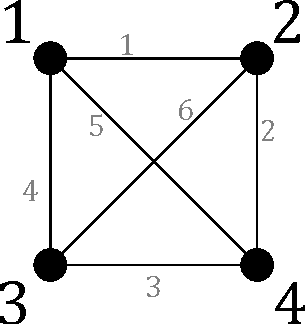
\includegraphics[scale=0.7]{figures/3_10_3-conn-6-edge.pdf} % edit %
            \caption{3-regular graph with 4 vertices}
            \label{fig:3_10}
        \end{figure}
    }
\end{enumerate}
